% Sun versus Clock — Paper A (TISMIR target)
% Draft v2 in a neutral article class; port to the venue class on submission.
% All numbers regenerate from the released notebooks
% (github.com/sudiptai/solar-samay-raga): Part A run of 12 Nov 2026 and
% Part B v6 run of 12 Nov 2026 (REAL mode, Saraga 1.5 Hindustani).
\documentclass[11pt]{article}
\usepackage[a4paper,margin=2.5cm]{geometry}
\usepackage{amsmath,amssymb}
\usepackage{graphicx}
\usepackage{booktabs}
\usepackage[numbers,sort&compress]{natbib}
\usepackage[hidelinks]{hyperref}
\usepackage{microtype}
\usepackage{appendix}

\newcommand{\todo}[1]{\textbf{[#1]}}

\title{Sun versus Clock: Formalizing the Hindustani Samay System on Solar
Phase and Measuring Its Divergence from the Fixed-Clock Convention}
\author{Sudipta Bhattacharya\\[2pt]
\small IEM Centre of Excellence for Cloud Computing and IoT,\\
\small Department of CSE (AIML) and CSBS, Institute of Engineering and Management,\\
\small Kolkata, West Bengal, India\\
\small \texttt{bhattacharya.sudipta@gmail.com}}
\date{Draft of November 12, 2026}

\begin{document}
\maketitle

\begin{abstract}
In Hindustani classical music, ragas carry prescribed performance windows
(\emph{samay}). The genuinely solar part of this prescription is the
\emph{sandhi-prakash} (twilight) class, anchored to sunrise and sunset, which
shift with latitude, longitude, and season, while prior computational
treatments of raga time assume a fixed clock. We propose a solar
formalization of the samay system: six window arcs defined on an
astronomically computed, season-invariant solar phase $\psi(t,\ell,d)$, with
the twilight arcs straddling the solar events, presented explicitly as a
modelling convention consistent with one reading of prahar reckoning. By
exact integration of the disagreement set, the fixed-clock convention and the
solar formalization assign different windows for 15.7\% of the day weighted
by state population (15.9\% under a 1-km population raster), rising to 35.9\%
at the western extreme in winter, with window onsets shifting
${\approx}81$ minutes between Kolkata and Srinagar under one time zone and
${\approx}80$ minutes across seasons at a single site. We release a unified,
source-cited raga--samay table (91 ragas with explicit anytime, seasonal, and
imported classes, reconciling disagreements in prior engineering sources).
On Saraga Hindustani, features derived from the corpus's expert melody and
tonic annotations (tonic-normalized cent-resolution pitch distributions)
identify ragas at $89.3\% \pm 5.1$ recording-level majority vote over 8
classes under leave-one-artist-out evaluation, above recording-level
permutation chance at $p \le 10^{-4}$ on every seed, and 13.1 points above a
12-bin pitch-class baseline; whether Bhatkhande's codified svara--samay
correlation is audible remains preliminary, because in this corpus most
time-windows are carried by a single raga, collapsing the window task into
raga identification. A closed-form identifiability analysis of the
formalization itself is confined to an appendix. We state plainly what the
framework does not yet show: recommendation value, performance-practice
claims, and affective claims await timestamped performance data and a
psychometric rating study, both specified herein.
\end{abstract}

\paragraph{Keywords.} Indian classical music; raga; samay; computational
musicology; solar time; music information retrieval; cultural analytics.

\section{Introduction}

Hindustani classical music assigns each raga a prescribed window in the
diurnal cycle. A listener at a morning concert expects Todi or Jaunpuri;
Yaman belongs to the first hours of night; Lalit announces the end of night.
This \emph{samay} (time) system, systematized in the early twentieth century
by V.~N.~Bhatkhande, has few parallels in other art-music traditions, and it
has begun to attract computational attention: Roy, Chakrabarty and
De~\cite{roy2017} trained a neural network to classify ragas into day and
night classes from symbolic features, using fixed clock windows such as
07:00--10:00.

This paper starts from an observation about that fixed clock. The part of the
samay system with the clearest physical referent is the
\emph{sandhi-prakash} class: the twilight ragas, defined by the transition of
light at dawn and dusk. Sunrise and sunset are functions of latitude,
longitude, and date. Across India, which spans roughly $29^\circ$ of
longitude under a single time zone, sunrise at the same IST clock instant
differs by nearly two hours between the eastern and western extremes; at one
site, it shifts by some 80 minutes between the solstices. A computational
model that encodes samay as fixed clock intervals therefore cannot be
simultaneously faithful to the tradition's twilight anchoring in Srinagar and
in Kolkata, in June and in December. The observation licenses less than it
may seem to. The tradition itself does not legislate per-location
astronomical recomputation: Bhatkhande states prahars and approximate clock
times, and All India Radio historically scheduled by clock. We therefore
propose solar anchoring as an explicit formalization, strongest for the
sandhi-prakash windows, and we quantify its divergence from the fixed-clock
convention rather than declaring either one correct.

Concretely, we make four contributions. \textbf{(i)}~A solar formalization of
samay: a season-invariant solar phase $\psi(t,\ell,d)$ computed from standard
solar-position equations, on which the six traditional performance windows
are defined as arcs, the twilight arcs straddling sunrise and sunset
(Section~\ref{sec:formal}). By exact integration, this formalization
disagrees with the fixed-clock convention for 15.7\% of the day weighted by
state population, 18.8\% on average across 13 cities spanning the extremes,
and up to 35.9\% in the far west in winter. \textbf{(ii)}~A unified,
source-cited raga--samay table of 91 ragas with explicit \emph{anytime},
\emph{light}, \emph{seasonal}, and \emph{imported} classes, reconciling
errors and inconsistencies we document in prior engineering sources
(Section~\ref{sec:table}). \textbf{(iii)}~A study on Saraga
Hindustani~\cite{saraga} with annotation-derived features under
leave-one-artist-out evaluation. Tonic-normalized cent-resolution pitch
distributions identify ragas at $89.3\% \pm 5.1$ recording-level majority
vote over 8 classes, with recording-level permutation $p \le 10^{-4}$ on
every seed, and the companion question, whether the codified svara--samay
correlation is audible, proves underdetermined in this corpus; we report it
as preliminary and state its confound (Section~\ref{sec:real}).
\textbf{(iv)}~A closed-form identifiability analysis establishing that the
formalization is recoverable from context features, with the Bayes-optimal
rule as the ceiling; because its labels are generated by the formalization
itself, it is a design check, not evidence, and it is confined to
Appendix~\ref{app:ident}.

Throughout, we treat the samay prescriptions as the tradition's normative
claims, not as established facts about listeners, and we treat samay in any
deployed system as a soft prior over a ranked list rather than a hard filter:
modern concert practice freely programs morning ragas at night, and Bhairavi
concludes concerts at any hour. The falsifiable version of this paper's
central premise, that solar-corrected samay predicts actually-programmed
ragas better than the fixed clock, requires timestamped performance data;
Section~\ref{sec:future} sets it out as the main direction for future work.

\section{Background and related work}\label{sec:related}

\paragraph{The samay system and its scholarship.}
The association of ragas with times of day is attested from the medieval
g\=ana-k\=ala rules of the \emph{Sa\.ng\=ita-Ratn\=akara} lineage, but the
system in modern use is substantially Bhatkhande's
rationalization~\cite{bhatkhande}: ragas are grouped by the position of the
v\=ad\=i (sonant) in p\=urv\=a\.nga or uttar\=a\.nga, by the flattened second
and sixth degrees that mark the sandhi-prakash (twilight) classes, and by the
madhyam as an indicator distinguishing day from night ragas. The two systems
differ materially and cannot be cited interchangeably. For our purposes the
important point is that the scholarship on the system (Jairazbhoy's analysis
of its internal logic~\cite{jairazbhoy}, Deva~\cite{deva}, Kaufmann's
per-raga compendium~\cite{kaufmann}, Bor et al.'s performance-time
listings~\cite{ragaguide}, and Clayton on time in Indian music
generally~\cite{clayton}) treats its rationale as conventional and contested,
and documents a persistent gap between prescription and modern concert
practice, in which evening programming dominates and the concluding raga
Bhairavi is sung at any hour. We therefore model samay as a normative
prescription whose structure can be formalized and whose observance is an
empirical question, not a ground truth.

\paragraph{Computational raga modelling.}
Raga recognition is a mature MIR task on CompMusic-lineage corpora:
pitch-class distributions~\cite{chordia2007}, fine-grained cent-resolution
pitch distributions with kernel density estimation~\cite{koduri2012},
time-delayed melody surfaces (TDMS)~\cite{gulati2016}, which remain the
standard strong baseline, and phrase- and deep-learning-based approaches. All
model raga identity from tonic-normalized pitch representations; none models
performance context such as time or place. The one computational treatment of
raga time, Roy et al.~\cite{roy2017}, classifies 23 ragas into two classes
(p\=urv\=a\.nga/uttar\=a\.nga rendered as day/night) from three symbolic
features under fixed clock windows; we document in Section~\ref{sec:table}
that several of its raga--window assignments do not survive comparison with
the musicological sources.

\paragraph{Context-aware recommendation and music emotion.}
Context-aware recommender systems have long modelled time and
location~\cite{adomavicius}, including for music~\cite{kaminskas}; our claim
is therefore scoped: location is unmodelled within computational raga
systems, not in music recommendation at large. Music emotion recognition
supplies mature machinery (categorical and dimensional valence-arousal
labels, benchmark protocols, and the finding that such labels require
controlled annotation~\cite{deam}), and raga-specific emotion has an
empirical literature of its own~\cite{mathur,balkwill,basu}. This paper makes
no affective claims: a psychometric rating study is specified as future work,
and the synthetic tokens used in the identifiability analysis of
Appendix~\ref{app:ident} are labelled as such wherever they appear.

\paragraph{The gap.}
Within computational raga modelling: (a)~time has been modelled only as a
fixed clock; (b)~location has not been modelled at all, although the
tradition's twilight anchor is a solar phenomenon that varies with location
and season; (c)~no unified, source-cited machine-readable raga--samay
resource existed. Sections~\ref{sec:formal}--\ref{sec:real} address
(a)--(c) in turn. \todo{Pre-submission: attach the documented search protocol
(databases, queries, dates) as supplementary material backing claim (b).}

\section{A solar formalization of samay}\label{sec:formal}

\paragraph{Solar phase.}
For a location $\ell = (\varphi, \lambda)$ (degrees, east-positive), date
with day-of-year $N$, and local clock time $t$ on a zone with reference
meridian $\lambda_{tz}$ (IST: $82.5^\circ$E), we use the standard
approximations for solar declination and the equation of time,
\begin{equation}
\delta(N)=23.44^{\circ}\sin\!\Big(\tfrac{360^{\circ}}{365}(N-81)\Big),
\qquad
E(N)=9.87\sin 2B-7.53\cos B-1.5\sin B,
\quad B=\tfrac{360^{\circ}}{365}(N-81),
\label{eq:decl}
\end{equation}
local solar time and the sunrise hour angle,
\begin{equation}
T_{\mathrm{sol}}=t+\frac{4(\lambda-\lambda_{tz})+E(N)}{60},
\qquad
\cos\omega_0=-\tan\varphi\tan\delta,
\qquad
D=\frac{2\omega_0}{15^{\circ}},\;\;\bar D=24-D,
\label{eq:sun}
\end{equation}
with sunrise/sunset at $12 \mp \omega_0/15$ in solar time ($\cos\omega_0$
clipped to $[-1,1]$; atmospheric refraction, about $0.83^\circ$ or 3--4
minutes, is an optional term, off in all experiments). The prahar index and
the season-invariant solar phase $\psi \in [0,1)$, with day mapped to
$[0,0.5)$ from sunrise and night to $[0.5,1)$ from sunset, follow as
\begin{equation}
\Pi=\begin{cases}
\big\lceil 4(T_{\mathrm{sol}}-t_{sr})/D\big\rceil, & \text{day}\\[2pt]
4+\big\lceil 4\Delta/\bar D\big\rceil,\;
\Delta=(T_{\mathrm{sol}}-t_{ss})\bmod 24, & \text{night}
\end{cases}
\qquad
\psi=\begin{cases}
\dfrac{T_{\mathrm{sol}}-t_{sr}}{2D}, & \text{day}\\[6pt]
\dfrac12+\dfrac{\Delta}{2\bar D}, & \text{night}
\end{cases}
\label{eq:psi}
\end{equation}
with model features $x_{\mathrm{time}} = [\sin 2\pi\psi,\, \cos 2\pi\psi,\,
\mathrm{onehot}(\Pi)]$. Equation~\eqref{eq:psi}'s quarter-of-daylight prahar
reading is one convention among several (pa\~nc\=a\.nga reckonings differ);
we adopt it as an explicit modelling choice, and Roy et al.'s two classes
correspond to $\Pi \in \{1\text{--}4\}$ vs $\{5\text{--}8\}$ by construction,
not as a validation. Against the full NOAA solar algorithm over a
$6\times6\times12$ grid spanning India, these approximations err by 0.9
minutes on average for sunrise (maximum 3.7) and 0.7 minutes for sunset
(maximum 2.5), negligible beside the window widths.

\paragraph{Window arcs.}
The six traditional windows are defined as arcs of $\psi$: dawn $[0.95,
0.04)$, morning $[0.04, 0.17)$, midday $[0.17, 0.42)$, dusk $[0.42, 0.55)$,
evening $[0.55, 0.70)$, night $[0.70, 0.95)$. The two sandhi-prakash arcs
straddle their solar events ($\psi = 0$ is sunrise, $\psi = 0.5$ sunset):
Lalit, Sohini, Paraj and Bhatiyar belong to the end of night, and Marwa and
Shree span sunset. A hard boundary at the solar instant would misplace
precisely the ragas whose anchoring is genuinely solar. ``Mid-morning'' thus
denotes the same phase in June and December, the invariance the prescription
intends, while the raw clock does not. Figure~\ref{fig:clock} shows the
resulting window geometry over a year at Kolkata against the fixed-clock
windows of prior work, and Figure~\ref{fig:onset} the spread of the first
prahar's onset across 13 cities under one IST clock.

\begin{figure}[t]
\centering
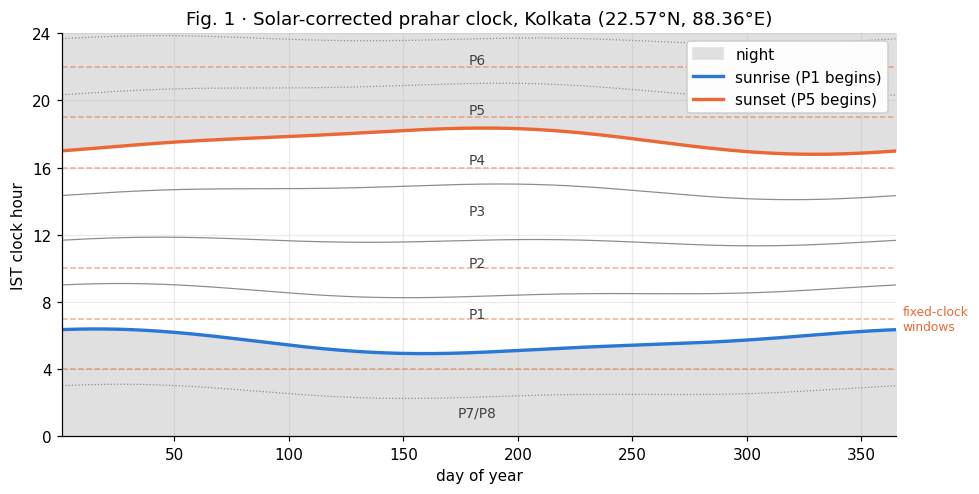
\includegraphics[width=.85\linewidth]{figs/partA_fig1.png}
\caption{The solar window geometry over a year at Kolkata
($22.57^\circ$N, $88.36^\circ$E). Solid curves: sunrise and sunset; the
eight prahar boundaries breathe with the seasons, while the fixed-clock
windows of prior work (dashed) stay frozen.}
\label{fig:clock}
\end{figure}

\begin{figure}[t]
\centering
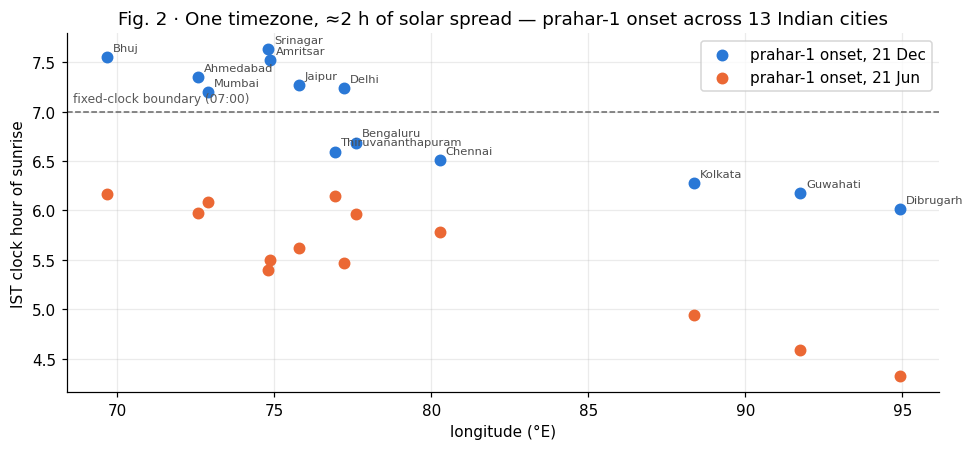
\includegraphics[width=.85\linewidth]{figs/partA_fig2.png}
\caption{One time zone, about two hours of solar spread: the onset of the
first prahar (sunrise) in IST clock time across 13 Indian cities at the two
solstices, against the 07:00 fixed-clock boundary of prior work.}
\label{fig:onset}
\end{figure}

\paragraph{Divergence between the two conventions.}
Neither the fixed-clock windows of prior work nor our solar arcs are
legislated by the tradition, so we quantify their disagreement rather than
declare error. The comparator is specified exactly: the fixed-clock
convention is the six IST windows of Roy et al.~\cite{roy2017} (dawn
04--07, morning 07--10, midday 10--16, dusk 16--19, evening 19--22, night
22--04), applied identically at every location and date; the solar
convention is the arc set above, fixed from prahar structure before this
comparison was run and not fitted to it. Because both conventions are
piecewise constant in clock time, their disagreement over a day is a union
of intervals delimited by at most twelve breakpoints (six clock boundaries
and six arc boundaries mapped to clock time), so we integrate it exactly
rather than sample it; an earlier grid-sampled figure was inflated by
boundary-aligned sampling, and the exact values replace it. Across 13
Indian cities $\times$ 12 months, the conventions assign different windows
for 18.8\% of the day on average (minimum 7.0\%, median 18.5\%, maximum
35.9\%, at Bhuj in February; Figure~\ref{fig:heatmap}). Two analytic facts
drive this: at the 21~December solstice, sunrise differs by 81 minutes
between Kolkata and Srinagar under one IST clock, and by 80 minutes at
Kolkata alone between solstices; the pure longitude span of India
contributes about 115 minutes (Table~\ref{tab:worked}). The 13-city sample
deliberately includes the geographic extremes. Weighted by state population
(Census 2011, 30 states represented by their capitals), the divergence is
15.7\% of the day, and re-weighting by a 1-km population
raster~\cite{worldpop} (1{,}127 aggregated cells above 50{,}000 people,
covering 1.38 billion) gives 15.9\%, so the state-capital approximation is
sound. Across states the figure ranges from 10.0\% (Odisha) to 24.4\%
(Gujarat). The headline is also not an artifact of any single boundary
choice: shifting each of the six arc boundaries by $\pm 0.02$ (about
$\pm 29$ minutes of a 12-hour day) moves the 13-city mean within
17.3--20.7\%. More than one hour in seven of the median Indian listener's
day is assigned differently by the two conventions: whatever one's reading
of samay, the choice is consequential, and the rest of the paper examines
that premise.

\begin{table}[t]
\centering
\caption{Worked example of the solar geometry (no refraction; all clock
times IST).}
\label{tab:worked}
\begin{tabular}{lccc}
\toprule
Site, date & Sunrise & Sunset & Daylight $D$ \\
\midrule
Kolkata, 21 Dec  & 06:17 & 16:54 & 10 h 37 m \\
Srinagar, 21 Dec & 07:38 & 17:21 & 9 h 43 m  \\
Kolkata, 21 Jun  & 04:56 & 18:20 & 13 h 24 m \\
\bottomrule
\end{tabular}
\end{table}

\begin{figure}[t]
\centering
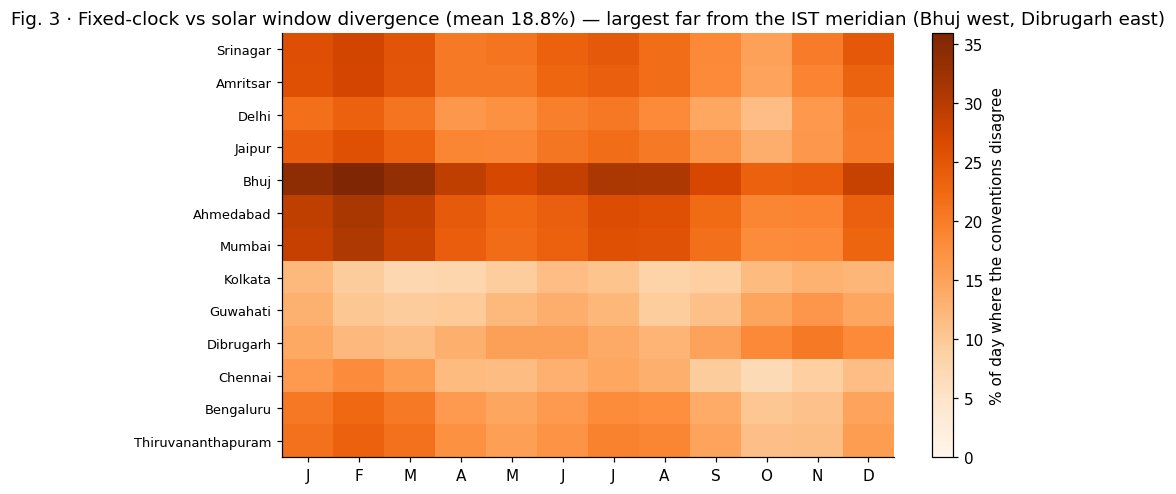
\includegraphics[width=.9\linewidth]{figs/partA_fig3.png}
\caption{Fixed-clock vs solar window divergence (\% of the day, exact
integration) per city and month. The divergence is largest far from the
$82.5^\circ$E IST meridian (Bhuj in the west, Dibrugarh in the east) and in
winter.}
\label{fig:heatmap}
\end{figure}

\section{A unified, source-cited raga--samay table}\label{sec:table}

Computational work on raga time has so far inherited its raga--window
assignments from engineering papers rather than musicological sources, and
the inherited tables contain errors a knowledgeable reader will catch
immediately: in~\cite{roy2017}, Gara (a light, thumri-a\.nga raga of the
evening) appears in the morning; Bhairavi, the sarva-k\=alika concluding raga
performed at any hour, is assigned to midday; Gaud Sarang (conventionally
early afternoon) to morning; Jaunpuri and Bilaskhani Todi (late morning) to
midday. We therefore built a unified table of 91 ragas, released as
machine-readable CSV, with per-raga sources (Bhatkhande's \emph{Kramik
Pustak M\=alik\=a}~\cite{bhatkhande}; Kaufmann~\cite{kaufmann}; Bor et
al.~\cite{ragaguide}) and a dispute-notes column recording where the sources
disagree.

Each raga carries a status: \emph{fixed} (60 ragas; time-supervisable),
\emph{anytime} (Bhairavi), \emph{light} (8: thumri-a\.nga vehicles such as
Pilu, Kafi, and Gara, flexible by practice), \emph{seasonal} (10: the Malhar
family, Basant and Bahar, the monsoon-associated Desh, and the spring Hindol,
where the seasonal association dominates the diurnal one), and
\emph{imported} (6: Carnatic and modern ragas such as Hansadhwani, Kirwani,
Abhogi, and Jog, whose ``times'' are modern concert habit rather than
traditional samay). Only \emph{fixed} ragas enter time-supervised
experiments; all statuses enter raga identification. Exclusion criteria are
thus applied uniformly, a consistency the earlier ad-hoc tables lacked. Where
our window assignment required adjudication (Durga and Shankara sit on the
evening/night discretization boundary; Maru Bihag, a raga distinct from Bihag
despite the name, keeps its own entry in the night class; Sohini is placed on
the pre-sunrise side of the dawn arc), the table records the decision and its
source rather than hiding it. Saraga's IAST-transliterated spellings are
resolved to table entries by diacritic-stripped matching plus an explicit
alias list, and every merge is an auditable editorial decision (for example,
Kaly\=a\d{n} to Yaman, and Todi to Miyan ki Todi). \todo{Pre-submission:
page-level references from library copies; worksheet in progress.}

\section{Experiments on Saraga Hindustani with annotation-derived
features}\label{sec:real}

\paragraph{Data and features.}
Saraga 1.5 Hindustani~\cite{saraga} has 108 concert recordings, of which 93
carry raga metadata resolving to 60 distinct ragas of the unified table (4
rare names remain unmapped and are listed in the released code). Ragas with
at least 3 recordings form the identification set: $N = 28$ recordings,
$K = 8$ ragas (Shree and Bhairavi 5 each; Yaman, Jog, Lalit, Marwa, Miyan
Malhar, and Miyan ki Todi 3 each), 8 distinct artists, 903 thirty-second
segments, 7.5 hours. A raga is defined by its svara material relative to the
tonic, so the features are tonic-normalized cent-resolution pitch
distributions: 120-bin folded histograms (10-cent resolution) computed from
Saraga's expert predominant-melody and ctonic annotations, plus a voicing
ratio. We say annotation-derived rather than audio-based advisedly: no
representation is learned from the waveform, and the results certify the
pipeline from expert melody annotations to raga identity, not an end-to-end
audio system. This is the representation family of the raga-recognition
literature~\cite{chordia2007,koduri2012,gulati2016}. It is intonation-aware
where 12-bin chroma is not, and it avoids the tabla and tanpura contamination
of full-mix spectral features. A speech SSL baseline (wav2vec
2.0~\cite{wav2vec}, mean-pooled) scored at chance on this corpus in a
preliminary run, the expected failure of a speech representation under small
per-class counts; we report it as a cautionary comparison, not a
contribution. A sanity check of the tonic annotations (histogram mass
concentrated at Sa and the fifth) flags none of the 28 recordings, so we cite
the ctonic files as verified.

\paragraph{Protocol.}
Evaluation is leave-one-artist-out (LOAO) over the 8 artists: in each fold,
every recording by the held-out artist is predicted by a model that has never
seen that performer, so performer voice and venue acoustics cannot leak; a
validation carve-out within each fold is itself artist-disjoint. Pooling the
folds predicts every recording exactly once. The primary metric is
recording-level majority vote over segment predictions, since the recording,
not the 30-second segment, is the musical unit; segment accuracy and
class-balanced segment accuracy are secondary. Segments from one recording
are statistically dependent, so segment-level permutation tests overstate
significance; chance is instead estimated by permuting recording labels
($10^4$ shuffles, $p = (c+1)/(n+1)$). The whole protocol is repeated over
three seeds, which vary initialization and the validation carve-out, and we
report mean $\pm$ sd.

\paragraph{Raga identification.}
Recording-level majority vote $89.3\% \pm 5.1$ (per-seed 85.7, 96.4, 85.7),
with recording-level permutation $p \le 10^{-4}$ on every seed against an
empirical chance of about 13.5\%; segment accuracy $74.0\% \pm 5.9$,
balanced $70.8\% \pm 6.6$. Figure~\ref{fig:conf} shows the pooled confusion.
Eight classes and 28 recordings make this a small study, and its value lies
in what it certifies: the field's standard representation, computed from
expert annotations under the strictest split in use, recovers raga identity
far above chance on an open corpus, and the same pipeline applies to larger
corpora without modification. Two further analyses support the
representation choice. Against the classic 12-bin pitch-class distribution
of Chordia and Rae~\cite{chordia2007}, computed from the same cached
histograms under the same LOAO protocol ($76.2\% \pm 4.5$ recording-level),
cent resolution adds 13.1 points; removing the voicing ratio changes nothing
($+0.0$), evidence that the feature is not smuggling in recording
conditions. The error analysis behaves as distribution features predict:
pooling segment errors over the three seeds (705 in all), 41\% fall in
scale-sharing allied pairs, led by Miyan ki Todi taken for Shree (128
errors; the two share komal re and tivra ma, and Miyan ki Todi's recall,
0.11 in the last seed, is the casualty), with Lalit--Marwa and
Bhairavi--Miyan ki Todi following; the largest confusion outside the listed
pairs, Miyan Malhar with Yaman in both directions, is not scale-based and
plausibly reflects the seasonal raga's heterogeneous melodic material.
Distribution features discard melodic order, so allied-raga confusion is the
expected failure mode, and sequence-aware baselines such as
TDMS~\cite{gulati2016} are the right next comparison.

\begin{figure}[t]
\centering
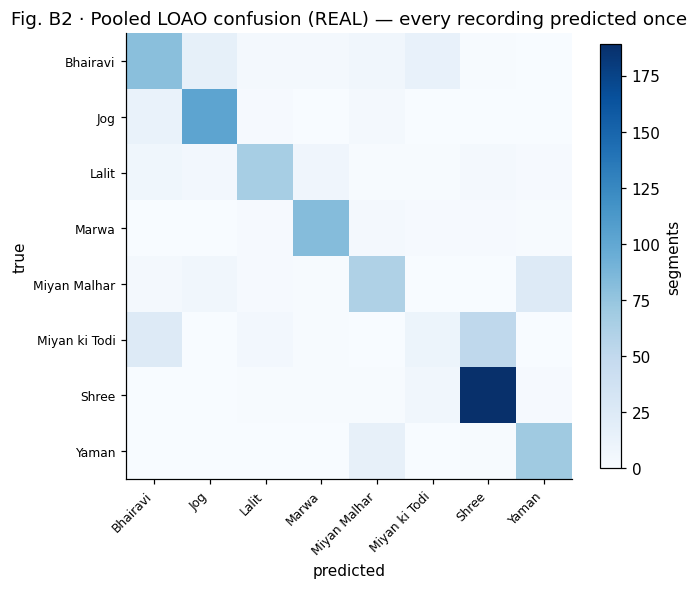
\includegraphics[width=.6\linewidth]{figs/partB_fig1.png}
\caption{Pooled LOAO segment confusion over the 8-raga identification set;
every recording is predicted by a model that never saw its artist. The
dominant off-diagonal mass is the allied pair Miyan ki Todi $\to$ Shree.}
\label{fig:conf}
\end{figure}

\paragraph{Is the svara--samay correlation audible? (preliminary).}
Bhatkhande's system correlates time-class with svara material by design:
komal re and dha mark the sandhi-prakash classes, and the madhyam separates
day from night ragas. One may therefore ask whether a classifier recovers a
raga's theoretical time-class from pitch content alone. This is a question
about the codification, not about when Saraga's concert recordings were
performed. On the fixed-status subset (17 recordings, 5 ragas, 4 windows)
the answer is underdetermined: $39.0\%$ mean top-1 with per-seed permutation
$p$ of $10^{-4}$, 0.002, and 0.92, and, decisively, three of the four
windows are carried by a single raga (dawn by Lalit, morning by Miyan ki
Todi, evening by Yaman), so the window task largely collapses into raga
identification (Figure~\ref{fig:b2}). We report this experiment as
preliminary with the confound stated, and identify the remedy (a corpus with
at least two ragas per window, Section~\ref{sec:future}) rather than
claiming the result.

\begin{figure}[t]
\centering
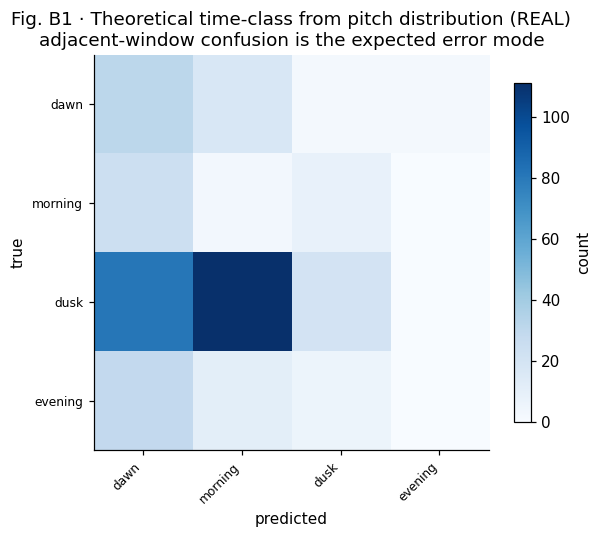
\includegraphics[width=.6\linewidth]{figs/partB_fig2.png}
\caption{Theoretical time-class from pitch distributions on Saraga
(preliminary; see text for the single-raga-window confound).}
\label{fig:b2}
\end{figure}

\paragraph{What we do not claim.}
No context-fusion result on real audio is reported. Saraga carries no
performance timestamps, and fusing audio with context sampled from the raga's
own canonical arc would constitute label leakage by construction. The
released notebook contains such a cell solely as a pipeline check, labelled
accordingly.

\section{Discussion}\label{sec:disc}

\paragraph{Prescription and practice.}
Any computational treatment of samay must face the fact that the prescription
is imperfectly observed. Concert life concentrates in the evening, broadcast
schedules have historically run by clock, and the tradition itself sanctions
exceptions: Bhairavi concludes at any hour, and seasonal ragas override the
diurnal cycle in season. We have therefore been careful to let the system's
structure and its observance come apart. The solar formalization
(Section~\ref{sec:formal}) models the structure; whether practice follows it
is an open empirical question that our framework makes testable but that
Saraga, lacking timestamps, cannot answer. For the same reason a deployed
selector must treat samay as a soft prior over a ranked list. Our reference
implementation returns probabilities, always admits the anytime class, and
never refuses a raga, since a system that forbade Todi at 8~p.m.\ would
contradict a century of concert practice while claiming to honour tradition.

\paragraph{Limitations.}
(i)~The identifiability analysis of Appendix~\ref{app:ident} recovers our own
construction; its value is sensitivity analysis, not validation. (ii)~The
Saraga study is small ($K = 8$, $N = 28$) and its time-class companion is
confounded by single-raga windows; both scale with corpus size, not with
method changes. (iii)~Its features derive from expert melody annotations, so
the result certifies the representation and protocol, not an end-to-end audio
system; predominant-melody extraction would have to replace the annotations
for deployment. (iv)~Distribution features discard melodic grammar
(\=aroha/avaroha, pakad, gamaka), so allied ragas sharing a scale set remain
hard, and sequence-aware baselines such as TDMS~\cite{gulati2016} are the
right next comparison. (v)~The quarter-of-daylight prahar reading and the arc
boundaries are conventions; the reported sensitivity band (17.3--20.7\% for
the 13-city mean under $\pm 0.02$ boundary shifts) should accompany any claim
built on them. (vi)~The 13-city divergence sample is unweighted and spans the
extremes by design; the population-weighted figures (15.7\% by state
capitals, 15.9\% by raster) are the representative ones. (vii)~No affective
claims are made anywhere: the rasa tokens of Appendix~\ref{app:ident} are
synthetic, and the rating-study protocol (enculturated listeners, navarasa
multi-label plus valence-arousal, inter-rater reliability thresholds) is
specified separately for the follow-up study.

\section{Future work and conclusion}\label{sec:future}

Three extensions would carry this work furthest. \textbf{(1)~Timestamped
performances.} Archival All India Radio broadcast schedules, printed festival
programmes (all-night events such as the Dover Lane Music Conference are
ideal, since they span every prahar), and timestamped concert videos would
supply real (raga, time, place) triples, enabling the falsifiable headline
test: does the solar formalization predict programming better than the fixed
clock? As a by-product they would give the first quantitative measurement of
samay observance in modern practice. \textbf{(2)~Corpus scale.} The
CompMusic Hindustani raga-recognition corpus (about 300 recordings, 30 ragas)
removes the single-raga-window confound, supports the TDMS baseline
comparison directly, and lifts $K$ to a size reviewers of raga recognition
expect. Carnatic corpora are not an appropriate extension, since Carnatic
practice largely does not observe time prescriptions.
\textbf{(3)~Validated emotion.} The psychometric rating study specified
alongside this paper would replace synthetic tokens with reliable rasa and
valence-arousal labels, restoring the affective axis to the framework on an
evidential footing.

\paragraph{Conclusion.}
We have given the Hindustani samay system an explicit solar formalization
anchored where the tradition itself is solar, the twilight ragas, and shown
by exact integration that the choice between this formalization and the
fixed-clock convention of prior computational work affects more than one
hour in seven of the median Indian listener's day. We have released the
first source-cited, machine-readable raga--samay table with uniform
treatment of anytime, light, seasonal, and imported ragas, and shown on an
open corpus that the standard tonic-normalized pitch representation,
computed from expert annotations, recovers raga identity far above chance
under leave-one-artist-out evaluation with recording-level significance
testing. We have tried to be equally clear about what the evidence does not
show: recovering one's own formalization validates no practice, synthetic
tokens are not emotions, annotation-derived features certify no end-to-end
system, and a window class carried by a single raga tests nothing.
Timestamped programming data and a listener rating study would cross that
line; both are specified here and ready to run.

\paragraph{Data and code availability.}
Both notebooks (solar/divergence; Saraga pipeline), the 91-raga table, and
all seeds are released at
\url{https://github.com/sudiptai/solar-samay-raga}. Every figure and number
in this paper regenerates from a single run of each notebook.

\appendix
\section{Identifiability of the formalization (simulation)}\label{app:ident}

\paragraph{Scope.}
This appendix asks a design question: if a system computed the features of
Section~\ref{sec:formal}, could it recover the raga prescribed by the
formalization? Queries are generated from the $\psi$-arcs and a synthetic
5-way rasa token, so the labels are a noisy function of the very variables
some encodings receive. Results therefore measure recoverability of our own
construction and the sensitivity of feature encodings; they say nothing
about music, listeners, or performance practice.

\paragraph{Design.}
20 \emph{fixed}-status ragas from the unified table (their corrected
windows), 13 cities, uniform day-of-year; each query samples a clock time
whose $\psi$ falls in the raga's arc at that place and date, and emits the
raga's token with probability 0.8 (else uniform). 6{,}000 queries per run,
70/15/15 splits stratified by raga, a two-hidden-layer network (64-32,
dropout 0.15, Adam, early stopping), and four encodings: raw clock
($\sin/\cos t$), clock+token, solar ($\sin/\cos\psi$, prahar one-hot,
lat/lon), solar+token. Paired contrasts are repeated over five
data-generation seeds, each redrawing queries, split, and initialization,
and are reported as mean $\pm$ Monte-Carlo standard error with sign
consistency; with $n = 5$ repetitions, rank tests have no resolution and are
omitted.

\paragraph{Closed-form references and results.}
Because the generative process is known, the right references are
closed-form rules, not learned baselines. The Bayes-optimal rule attains
0.611 top-1 (0.972 top-3) on the reference run; a lookup rule (ragas whose
arc contains $\psi$, filtered by token, ties broken at random) attains 0.634
on one draw, but over 300 tie-breaking redraws it scores $0.619 \pm 0.012$
(range 0.589--0.656), a distribution that contains the Bayes rule: the two
are tie-breaking variants of one optimal family, and any single-test-set
ordering between them is noise. The network's encodings score 0.254 (clock),
0.586 (clock+token), 0.307 (solar), and 0.619 top-1 / 0.957 top-3
(solar+token) on the reference run; the full model thus matches the
closed-form optimum, and in simulation the learning component contributes
nothing beyond recovering the known rule, as expected. Paired over five
seeds, the token adds $+31.0 \pm 0.4$ points top-1 (a measurement of the
simulator's noise parameter, reported only as such), and the solar encoding
adds $+3.9 \pm 0.7$ with the token and $+4.2 \pm 0.4$ without; every
contrast is positive in all five seeds and exceeds twice its Monte-Carlo
standard error. Per-city gains are descriptive only: an apparent correlation
between gain and distance from the IST meridian in an earlier version
vanished under seed-averaging ($r = 0.00$, $p = 0.99$; mean gain $+4.4$
points for cities more than $6^\circ$ from the meridian versus $+4.0$
within). The gap between top-1 (0.619) and top-3 (0.957) reflects that
several ragas legitimately share an arc and token; the task is many-to-one
by design, which is why Section~\ref{sec:disc} frames deployment as ranked
selection under a soft prior.

\begin{table}[h]
\centering
\caption{Identifiability simulation, reference run (20 ragas; the ``token''
is synthetic, not an emotion label), with closed-form references. Paired
contrasts over five seeds appear in the text.}
\label{tab:feas}
\begin{tabular}{lccc}
\toprule
Encoding & Top-1 & Macro-F1 & Top-3 \\
\midrule
clock            & 0.254 & 0.180 & 0.748 \\
clock + token    & 0.586 & 0.540 & 0.938 \\
solar            & 0.307 & 0.224 & 0.849 \\
solar + token    & 0.619 & 0.584 & 0.957 \\
\midrule
rule lookup (expected over tie-breaks) & $0.619 \pm 0.012$ & -- & -- \\
Bayes-optimal (no learning)            & 0.611 & -- & 0.972 \\
\bottomrule
\end{tabular}
\end{table}

\begin{thebibliography}{20}
\bibitem{roy2017} S.~Roy, S.~Chakrabarty, and D.~De, ``Time-based raga
recommendation and information retrieval of musical patterns in Indian
classical music using neural networks,'' \emph{IAES Int.\ J.\ of Artificial
Intelligence}, 6(1):33--48, 2017.
\bibitem{bhatkhande} V.~N.~Bhatkhande, \emph{Hindusth\=an\=i Sa\.ng\=it
Paddhati: Kramik Pustak M\=alik\=a}, 6 vols. \todo{edition/publisher/year of
the copy cited.}
\bibitem{jairazbhoy} N.~A.~Jairazbhoy, \emph{The R\=ags of North Indian
Music: Their Structure and Evolution}. Faber, 1971.
\bibitem{deva} B.~C.~Deva, \emph{The Music of India: A Scientific Study}.
Munshiram Manoharlal, 1981.
\bibitem{kaufmann} W.~Kaufmann, \emph{The Ragas of North India}. Indiana
University Press, 1968.
\bibitem{ragaguide} J.~Bor, S.~Rao, W.~van der Meer, and J.~Harvey,
\emph{The Raga Guide: A Survey of 74 Hindustani Ragas}. Nimbus Records with
Rotterdam Conservatory, 1999.
\bibitem{clayton} M.~Clayton, \emph{Time in Indian Music}. Oxford University
Press, 2000.
\bibitem{chordia2007} P.~Chordia and A.~Rae, ``Raag recognition using
pitch-class and pitch-class dyad distributions,'' in \emph{Proc.\ ISMIR},
2007.
\bibitem{koduri2012} G.~K.~Koduri, S.~Gulati, P.~Rao, and X.~Serra,
``R\=aga recognition based on pitch distribution methods,'' \emph{J.\ New
Music Research}, 41(4):337--350, 2012.
\bibitem{gulati2016} S.~Gulati, J.~Serr\`a, K.~K.~Ganguli, S.~\c{S}ent\"urk,
and X.~Serra, ``Time-delayed melody surfaces for r\=aga recognition,'' in
\emph{Proc.\ ISMIR}, 2016.
\bibitem{deam} A.~Aljanaki, Y.-H.~Yang, and M.~Soleymani, ``Developing a
benchmark for emotional analysis of music,'' \emph{PLOS ONE},
12(3):e0173392, 2017.
\bibitem{saraga} A.~Srinivasamurthy, S.~Gulati, R.~Caro Repetto, and
X.~Serra, ``Saraga: open datasets for research on Indian art music.''
\todo{exact venue and year (2020/2021).}
\bibitem{adomavicius} G.~Adomavicius and A.~Tuzhilin, ``Context-aware
recommender systems,'' in \emph{Recommender Systems Handbook}. Springer.
\todo{edition/year.}
\bibitem{kaminskas} M.~Kaminskas and F.~Ricci, ``Contextual music
information retrieval and recommendation: state of the art and challenges,''
\emph{Computer Science Review}, 6(2--3):89--119, 2012.
\bibitem{mathur} A.~Mathur, S.~H.~Vijayakumar, B.~Chakrabarti, and
N.~C.~Singh, ``Emotional responses to Hindustani raga music: the role of
musical structure,'' \emph{Frontiers in Psychology}, 6:513, 2015.
\bibitem{balkwill} L.-L.~Balkwill and W.~F.~Thompson, ``A cross-cultural
investigation of the perception of emotion in music,'' \emph{Music
Perception}, 17(1):43--64, 1999.
\bibitem{basu} M.~Basu et al., \todo{full author list and exact title},
\emph{Physica A}, 624:128937, 2023.
\bibitem{mirdata} R.~M.~Bittner et al., ``mirdata: software for reproducible
usage of datasets,'' in \emph{Proc.\ ISMIR}, 2019.
\bibitem{wav2vec} A.~Baevski, H.~Zhou, A.~Mohamed, and M.~Auli, ``wav2vec
2.0: a framework for self-supervised learning of speech representations,''
in \emph{Proc.\ NeurIPS}, 2020.
\bibitem{worldpop} WorldPop, ``India 1~km population count, 2020,
UN-adjusted (ind\_ppp\_2020\_1km\_Aggregated\_UNadj),'' University of
Southampton. \url{https://www.worldpop.org}.
\end{thebibliography}

\end{document}
